\usetikzlibrary{arrows.meta,calc,shadings,fadings}

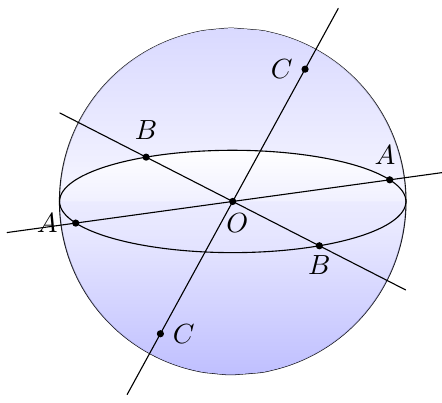
\begin{tikzpicture}[>=Stealth, line cap=round, line join=round]

% ----------------------------
% PARAMETERS
% ----------------------------
\def\a{2.2}       % ellipse x radius
\def\b{0.65}      % ellipse y radius
\def\H{2.2}       % hemisphere height
\def\Oy{-2.0}     % ground level y

\coordinate (O) at (0,\Oy);
\coordinate (Top) at (0,{\Oy+\H});   % equator center (flat top)

% ----------------------------
% ANGLES for labeled points
% ----------------------------
\def\phiA{25}     % azimuthal angle for A pair
\def\phiB{120}    % azimuthal angle for B pair

% ----------------------------
% SOUTHERN HEMISPHERE (dome down, equator on top)
% ----------------------------

% Silhouette meridians (one continuous path, no gap at bottom)
\draw
  plot[domain=0:1, samples=80, smooth]
  ({-\a*sqrt(1 - \x*\x)}, {\Oy + \H - \H*\x})
  -- plot[domain=1:0, samples=80, smooth]
  ({\a*sqrt(1 - \x*\x)}, {\Oy + \H - \H*\x});

% Fill with path fading
\fill[blue!25, path fading=north]
  plot[domain=0:1, samples=80, smooth]
  ({-\a*sqrt(1 - \x*\x)}, {\Oy + \H - \H*\x})
  -- (0, \Oy)
  -- plot[domain=1:0, samples=80, smooth]
  ({\a*sqrt(1 - \x*\x)}, {\Oy + \H - \H*\x})
  -- plot[domain=0:360, samples=80, smooth]
  ({\a*cos(\x)}, {\Oy + \H + \b*sin(\x)})
  -- cycle;

% ----------------------------
% NORTHERN HEMISPHERE (dome up, from equator)
% ----------------------------

% Silhouette meridians (north)
\draw
  plot[domain=0:1, samples=80, smooth]
  ({-\a*sqrt(1 - \x*\x)}, {\Oy + \H + \H*\x})
  -- plot[domain=1:0, samples=80, smooth]
  ({\a*sqrt(1 - \x*\x)}, {\Oy + \H + \H*\x});

% Fill northern hemisphere (fading south = transparent at top)
\fill[blue!15, path fading=south]
  plot[domain=0:1, samples=80, smooth]
  ({-\a*sqrt(1 - \x*\x)}, {\Oy + \H + \H*\x})
  -- (0, {\Oy + 2*\H})
  -- plot[domain=1:0, samples=80, smooth]
  ({\a*sqrt(1 - \x*\x)}, {\Oy + \H + \H*\x})
  -- plot[domain=0:360, samples=80, smooth]
  ({\a*cos(\x)}, {\Oy + \H + \b*sin(\x)})
  -- cycle;

% Equator ellipse
\draw
  plot[domain=0:360, samples=80, smooth]
  ({\a*cos(\x)}, {\Oy + \H + \b*sin(\x)});

% ----------------------------
% POINTS ON EQUATOR
% ----------------------------

% A pair
\coordinate (eqA)  at ({\a*cos(\phiA)}, {\Oy+\H+\b*sin(\phiA)});
\coordinate (eqA2) at ({-\a*cos(\phiA)}, {\Oy+\H-\b*sin(\phiA)});

% B pair
\coordinate (eqB)  at ({\a*cos(\phiB)}, {\Oy+\H+\b*sin(\phiB)});
\coordinate (eqB2) at ({-\a*cos(\phiB)}, {\Oy+\H-\b*sin(\phiB)});

% Solid lines: diametrically opposite on equator (extended beyond sphere)
\draw[shorten >=-25pt, shorten <=-25pt] (eqA) -- (eqA2);
\draw[shorten >=-35pt, shorten <=-35pt] (eqB) -- (eqB2);

% ----------------------------
% POINT C ON HEMISPHERE SURFACE
% ----------------------------
\pgfmathsetmacro{\tC}{0.55}       % t parameter (0=equator, 1=south pole)
\pgfmathsetmacro{\phiC}{-120}     % azimuthal angle
\coordinate (C) at
  ({\a*sqrt(1-\tC*\tC)*cos(\phiC)},
   {\Oy + \H - \H*\tC + \b*sqrt(1-\tC*\tC)*sin(\phiC)});

\fill (C) circle (1.3pt);
\node[right=1pt] at (C) {$C$};

% Diametrically opposite of C (in northern hemisphere)
\coordinate (C2) at
  ({-\a*sqrt(1-\tC*\tC)*cos(\phiC)},
   {\Oy + \H + \H*\tC - \b*sqrt(1-\tC*\tC)*sin(\phiC)});

\fill (C2) circle (1.3pt);
\node[left=1pt] at (C2) {$C$};

% Solid line C -- C (extended beyond sphere)
\draw[shorten >=-25pt, shorten <=-25pt] (C) -- (C2);

% ----------------------------
% CENTER POINT O
% ----------------------------
\fill (Top) circle (1.3pt);
\node[below=1pt] at (Top) {$\,\,O$};

% ----------------------------
% LABELS
% ----------------------------
\fill (eqA) circle (1.3pt);
\node[above=2pt] at (eqA) {$A\,\,$};
\fill (eqA2) circle (1.3pt);
\node[left=3pt] at (eqA2) {$A$};

\fill (eqB) circle (1.3pt);
\node[above=3pt] at (eqB) {$B$};
\fill (eqB2) circle (1.3pt);
\node[below=0pt] at (eqB2) {$B$};

\end{tikzpicture}